\documentclass{article}
\usepackage{booktabs}  % 用于表格 midrule
\usepackage{multirow}  % for multirow command used in the table
\usepackage{amssymb}  % 用于打对号
%\usepackage[UTF8]{ctex} % 用于写中文
\usepackage{geometry} % 用于调整页边距
\usepackage{graphicx}  % 用于 includegraphics
\begin{document}
\begin{table}[t]
    \centering
    \caption{Attack performance using the random pattern.
    The attack performance is evaluated according to AO/SR on GOT-Val.}
    \label{table:random}
    \begin{tabular}{@{}rcccc@{}}
    \toprule
    \multirow{2}{*}[-1pt]{\begin{tabular}[c]{@{}c@{}}Perturbations used to \\ perfrom attack \end{tabular}} & \multicolumn{2}{c}{Untargeted Attack} & \multicolumn{2}{c}{Targeted Attack}\\ \cmidrule{2-5}
                                                           & AO                                      & SR                               & AO                & SR                  \\ \midrule
    Trained Perturbations                                             & 0.153                                   & 0.123                            & 0.840             & 0.890               \\
    Random Pattern                                         & 0.736                                   & 0.871                            & 0.153             & 0.118               \\ \bottomrule        
    \end{tabular}
  \end{table}

\begin{figure}[t]
    \centering
    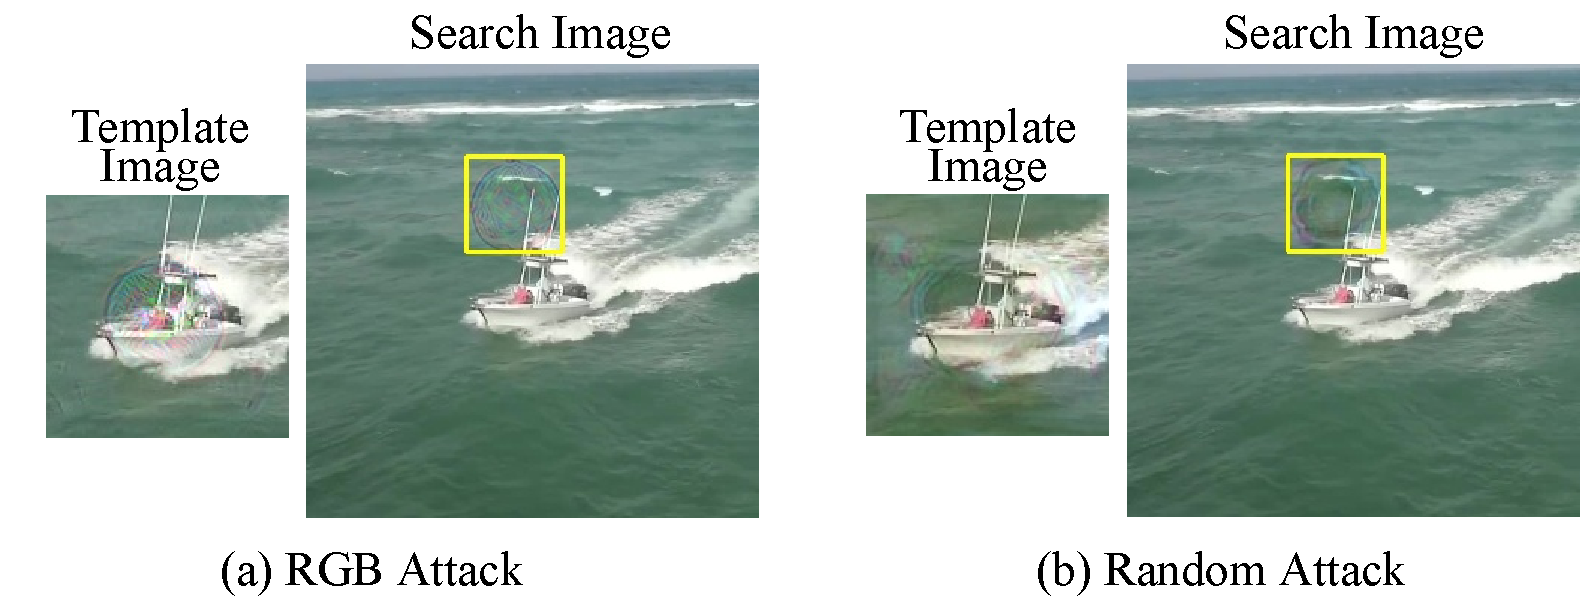
\includegraphics[width=0.8\textwidth]{random.pdf}
    \caption{Visualization of the random pattern.}
    \label{fig:random}
\end{figure}

Untargeted AO, SR:
0.7355267789379769, 0.8707800327017409

Targeted AO, SR:
0.15291608894028702, 0.11806290276041166

\end{document}